\documentclass[11pt]{article}

\usepackage[utf8]{inputenc}
\usepackage{changepage}
\usepackage{amsmath}
\usepackage{amsfonts}
\usepackage{amssymb}
\usepackage{url}
\usepackage{indentfirst}
\usepackage{hanging}
\usepackage{titlesec}
\usepackage{hyperref}
\usepackage{graphicx}

\setlength{\parindent}{0pt}
\setlength{\parskip}{0.5\baselineskip}

\renewcommand{\labelitemi}{\(\hookrightarrow\)}
\setlength{\itemsep}{0pt}
\titleformat{\section}{\bfseries\Large}{\thesection}{1em}{}
\titleformat{\subsection}{\bfseries\large}{\thesubsection}{1em}{}

\title{the least effective anti-ai literature for mathematicians}
\date{2026-10-12}
\begin{document}
\maketitle

Like I guess there is no reason to believe anyone would find this 1959 literary theory essay compelling or relevant but consider:

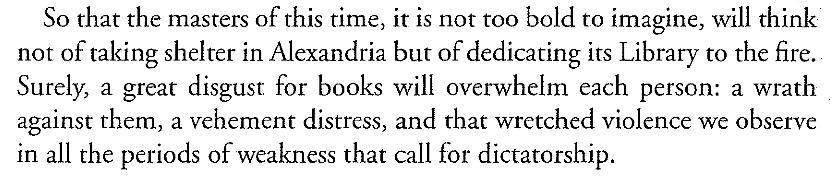
\includegraphics[width=70ex]{20261012-123202.png}

{\scriptsize Blanchot, Maurice. ``Death of the Last Writer.'' translated by Charlotte Mandell. in {\itshape The Book to Come}. 2003 [1959].}

\end{document}

